\documentclass[twoside]{book}

% Packages required by doxygen
\usepackage{fixltx2e}
\usepackage{calc}
\usepackage{doxygen}
\usepackage[export]{adjustbox} % also loads graphicx
\usepackage{graphicx}
\usepackage[utf8]{inputenc}
\usepackage{makeidx}
\usepackage{multicol}
\usepackage{multirow}
\PassOptionsToPackage{warn}{textcomp}
\usepackage{textcomp}
\usepackage[nointegrals]{wasysym}
\usepackage[table]{xcolor}

% Font selection
\usepackage[T1]{fontenc}
\usepackage[scaled=.90]{helvet}
\usepackage{courier}
\usepackage{amssymb}
\usepackage{sectsty}
\renewcommand{\familydefault}{\sfdefault}
\allsectionsfont{%
  \fontseries{bc}\selectfont%
  \color{darkgray}%
}
\renewcommand{\DoxyLabelFont}{%
  \fontseries{bc}\selectfont%
  \color{darkgray}%
}
\newcommand{\+}{\discretionary{\mbox{\scriptsize$\hookleftarrow$}}{}{}}

% Page & text layout
\usepackage{geometry}
\geometry{%
  a4paper,%
  top=2.5cm,%
  bottom=2.5cm,%
  left=2.5cm,%
  right=2.5cm%
}
\tolerance=750
\hfuzz=15pt
\hbadness=750
\setlength{\emergencystretch}{15pt}
\setlength{\parindent}{0cm}
\setlength{\parskip}{3ex plus 2ex minus 2ex}
\makeatletter
\renewcommand{\paragraph}{%
  \@startsection{paragraph}{4}{0ex}{-1.0ex}{1.0ex}{%
    \normalfont\normalsize\bfseries\SS@parafont%
  }%
}
\renewcommand{\subparagraph}{%
  \@startsection{subparagraph}{5}{0ex}{-1.0ex}{1.0ex}{%
    \normalfont\normalsize\bfseries\SS@subparafont%
  }%
}
\makeatother

% Headers & footers
\usepackage{fancyhdr}
\pagestyle{fancyplain}
\fancyhead[LE]{\fancyplain{}{\bfseries\thepage}}
\fancyhead[CE]{\fancyplain{}{}}
\fancyhead[RE]{\fancyplain{}{\bfseries\leftmark}}
\fancyhead[LO]{\fancyplain{}{\bfseries\rightmark}}
\fancyhead[CO]{\fancyplain{}{}}
\fancyhead[RO]{\fancyplain{}{\bfseries\thepage}}
\fancyfoot[LE]{\fancyplain{}{}}
\fancyfoot[CE]{\fancyplain{}{}}
\fancyfoot[RE]{\fancyplain{}{\bfseries\scriptsize Generated by Doxygen }}
\fancyfoot[LO]{\fancyplain{}{\bfseries\scriptsize Generated by Doxygen }}
\fancyfoot[CO]{\fancyplain{}{}}
\fancyfoot[RO]{\fancyplain{}{}}
\renewcommand{\footrulewidth}{0.4pt}
\renewcommand{\chaptermark}[1]{%
  \markboth{#1}{}%
}
\renewcommand{\sectionmark}[1]{%
  \markright{\thesection\ #1}%
}

% Indices & bibliography
\usepackage{natbib}
\usepackage[titles]{tocloft}
\setcounter{tocdepth}{3}
\setcounter{secnumdepth}{5}
\makeindex

% Hyperlinks (required, but should be loaded last)
\usepackage{ifpdf}
\ifpdf
  \usepackage[pdftex,pagebackref=true]{hyperref}
\else
  \usepackage[ps2pdf,pagebackref=true]{hyperref}
\fi
\hypersetup{%
  colorlinks=true,%
  linkcolor=blue,%
  citecolor=blue,%
  unicode%
}

% Custom commands
\newcommand{\clearemptydoublepage}{%
  \newpage{\pagestyle{empty}\cleardoublepage}%
}

\usepackage{caption}
\captionsetup{labelsep=space,justification=centering,font={bf},singlelinecheck=off,skip=4pt,position=top}

%===== C O N T E N T S =====

\begin{document}

% Titlepage & ToC
\hypersetup{pageanchor=false,
             bookmarksnumbered=true,
             pdfencoding=unicode
            }
\pagenumbering{roman}
\begin{titlepage}
\vspace*{7cm}
\begin{center}%
{\Large My Project \\[1ex]\large 1.\+0 }\\
\vspace*{1cm}
{\large Generated by Doxygen 1.8.11}\\
\end{center}
\end{titlepage}
\clearemptydoublepage
\tableofcontents
\clearemptydoublepage
\pagenumbering{arabic}
\hypersetup{pageanchor=true}

%--- Begin generated contents ---
\chapter{Class Index}
\section{Class List}
Here are the classes, structs, unions and interfaces with brief descriptions\+:\begin{DoxyCompactList}
\item\contentsline{section}{\hyperlink{classAStar}{A\+Star} \\*Defines the \hyperlink{classAStar}{A\+Star} class }{\pageref{classAStar}}{}
\item\contentsline{section}{\hyperlink{classMap}{Map} \\*Defines the \hyperlink{classMap}{Map} class }{\pageref{classMap}}{}
\item\contentsline{section}{\hyperlink{classNode}{Node} \\*Defines the \hyperlink{classNode}{Node} class }{\pageref{classNode}}{}
\end{DoxyCompactList}

\chapter{File Index}
\section{File List}
Here is a list of all documented files with brief descriptions\+:\begin{DoxyCompactList}
\item\contentsline{section}{app/\hyperlink{AStar_8cpp}{A\+Star.\+cpp} \\*Implements A$\ast$ algorithm }{\pageref{AStar_8cpp}}{}
\item\contentsline{section}{app/\hyperlink{Map_8cpp}{Map.\+cpp} \\*Implements map class }{\pageref{Map_8cpp}}{}
\item\contentsline{section}{app/\hyperlink{Node_8cpp}{Node.\+cpp} \\*Implements node class }{\pageref{Node_8cpp}}{}
\item\contentsline{section}{include/\hyperlink{AStar_8h}{A\+Star.\+h} \\*Contains declarations for \hyperlink{classAStar}{A\+Star} class }{\pageref{AStar_8h}}{}
\item\contentsline{section}{include/\hyperlink{Map_8h}{Map.\+h} \\*Contains Declarations for \hyperlink{classMap}{Map} Class }{\pageref{Map_8h}}{}
\item\contentsline{section}{include/\hyperlink{Node_8h}{Node.\+h} \\*Contains declarations for \hyperlink{classNode}{Node} class }{\pageref{Node_8h}}{}
\item\contentsline{section}{test/\hyperlink{test_8cpp}{test.\+cpp} \\*Contains Unit tests }{\pageref{test_8cpp}}{}
\end{DoxyCompactList}

\chapter{Class Documentation}
\hypertarget{classAStar}{}\section{A\+Star Class Reference}
\label{classAStar}\index{A\+Star@{A\+Star}}


Defines the \hyperlink{classAStar}{A\+Star} class.  




{\ttfamily \#include $<$A\+Star.\+h$>$}

\subsection*{Public Member Functions}
\begin{DoxyCompactItemize}
\item 
\hyperlink{classAStar_a0903f971fd29f74179cf269db934a469}{A\+Star} (int \+\_\+startx, int \+\_\+starty, int \+\_\+goalx, int \+\_\+goaly)
\begin{DoxyCompactList}\small\item\em Constructor for initializing goal and start coordinates. \end{DoxyCompactList}\item 
std\+::vector$<$ int $>$ \hyperlink{classAStar_aa63c6af8c1c0fa4f422775e75ba61c35}{path\+Find} (std\+::vector$<$ std\+::vector$<$ int $>$ $>$ vec)
\begin{DoxyCompactList}\small\item\em finds the path of directions from start to goal \end{DoxyCompactList}\end{DoxyCompactItemize}
\subsection*{Public Attributes}
\begin{DoxyCompactItemize}
\item 
int {\bfseries startx}\hypertarget{classAStar_a7beab7460a53378df536e95d36926082}{}\label{classAStar_a7beab7460a53378df536e95d36926082}

\item 
int {\bfseries starty}\hypertarget{classAStar_a63e9ef8b8a53b36084cc496d9f765415}{}\label{classAStar_a63e9ef8b8a53b36084cc496d9f765415}

\item 
int {\bfseries goalx}\hypertarget{classAStar_aed7140142494cdae9d05ef4f01349c5f}{}\label{classAStar_aed7140142494cdae9d05ef4f01349c5f}

\item 
int {\bfseries goaly}\hypertarget{classAStar_a02edb859e745c730e450e9f18be7f90b}{}\label{classAStar_a02edb859e745c730e450e9f18be7f90b}

\end{DoxyCompactItemize}
\subsection*{Friends}
\begin{DoxyCompactItemize}
\item 
bool \hyperlink{classAStar_a1ac82d7bfc70d9941cc1e12baf250b75}{operator$>$} (const \hyperlink{classNode}{Node} \&, const \hyperlink{classNode}{Node} \&)
\begin{DoxyCompactList}\small\item\em overloads the \textquotesingle{}$>$\textquotesingle{} operator \end{DoxyCompactList}\end{DoxyCompactItemize}


\subsection{Detailed Description}
Defines the \hyperlink{classAStar}{A\+Star} class. 


\begin{DoxyParams}{Parameters}
{\em startx} & is the x coordinate of the start node \\
\hline
{\em starty} & is the y coordinate of the start node \\
\hline
{\em goalx} & is the x coordinate of the goal node \\
\hline
{\em goaly} & is the x coordinate of the goal node\\
\hline
\end{DoxyParams}
\begin{DoxyReturn}{Returns}
none 
\end{DoxyReturn}


\subsection{Constructor \& Destructor Documentation}
\index{A\+Star@{A\+Star}!A\+Star@{A\+Star}}
\index{A\+Star@{A\+Star}!A\+Star@{A\+Star}}
\subsubsection[{\texorpdfstring{A\+Star(int \+\_\+startx, int \+\_\+starty, int \+\_\+goalx, int \+\_\+goaly)}{AStar(int _startx, int _starty, int _goalx, int _goaly)}}]{\setlength{\rightskip}{0pt plus 5cm}A\+Star\+::\+A\+Star (
\begin{DoxyParamCaption}
\item[{int}]{\+\_\+startx, }
\item[{int}]{\+\_\+starty, }
\item[{int}]{\+\_\+goalx, }
\item[{int}]{\+\_\+goaly}
\end{DoxyParamCaption}
)}\hypertarget{classAStar_a0903f971fd29f74179cf269db934a469}{}\label{classAStar_a0903f971fd29f74179cf269db934a469}


Constructor for initializing goal and start coordinates. 

intitializes the coordinates of start \& goal coordinates 

\subsection{Member Function Documentation}
\index{A\+Star@{A\+Star}!path\+Find@{path\+Find}}
\index{path\+Find@{path\+Find}!A\+Star@{A\+Star}}
\subsubsection[{\texorpdfstring{path\+Find(std\+::vector$<$ std\+::vector$<$ int $>$ $>$ vec)}{pathFind(std::vector< std::vector< int > > vec)}}]{\setlength{\rightskip}{0pt plus 5cm}std\+::vector$<$ int $>$ A\+Star\+::path\+Find (
\begin{DoxyParamCaption}
\item[{std\+::vector$<$ std\+::vector$<$ int $>$ $>$}]{vec}
\end{DoxyParamCaption}
)}\hypertarget{classAStar_aa63c6af8c1c0fa4f422775e75ba61c35}{}\label{classAStar_aa63c6af8c1c0fa4f422775e75ba61c35}


finds the path of directions from start to goal 


\begin{DoxyParams}{Parameters}
{\em vec} & is a map which holds info if a node is walkable or blocked\\
\hline
\end{DoxyParams}
\begin{DoxyReturn}{Returns}
path with parent directions from start to goal 
\end{DoxyReturn}


\subsection{Friends And Related Function Documentation}
\index{A\+Star@{A\+Star}!operator$>$@{operator$>$}}
\index{operator$>$@{operator$>$}!A\+Star@{A\+Star}}
\subsubsection[{\texorpdfstring{operator$>$}{operator>}}]{\setlength{\rightskip}{0pt plus 5cm}bool operator$>$ (
\begin{DoxyParamCaption}
\item[{const {\bf Node} \&}]{p, }
\item[{const {\bf Node} \&}]{q}
\end{DoxyParamCaption}
)\hspace{0.3cm}{\ttfamily [friend]}}\hypertarget{classAStar_a1ac82d7bfc70d9941cc1e12baf250b75}{}\label{classAStar_a1ac82d7bfc70d9941cc1e12baf250b75}


overloads the \textquotesingle{}$>$\textquotesingle{} operator 

gives priority to node with greater total cosr


\begin{DoxyParams}{Parameters}
{\em p} & is a reference of a node \\
\hline
{\em q} & is a reference of a node\\
\hline
\end{DoxyParams}
\begin{DoxyReturn}{Returns}
true if the total cost of p is greater, else false 
\end{DoxyReturn}


The documentation for this class was generated from the following files\+:\begin{DoxyCompactItemize}
\item 
include/\hyperlink{AStar_8h}{A\+Star.\+h}\item 
app/\hyperlink{AStar_8cpp}{A\+Star.\+cpp}\end{DoxyCompactItemize}

\hypertarget{classMap}{}\section{Map Class Reference}
\label{classMap}\index{Map@{Map}}


Defines the \hyperlink{classMap}{Map} class.  




{\ttfamily \#include $<$Map.\+h$>$}

\subsection*{Public Member Functions}
\begin{DoxyCompactItemize}
\item 
std\+::vector$<$ std\+::vector$<$ int $>$ $>$ \hyperlink{classMap_ab0ba13c90105c4ad77814d4cfb6a35ab}{create\+Map} ()
\begin{DoxyCompactList}\small\item\em creates a 10x10 map with obstacles placed randomly \end{DoxyCompactList}\item 
int \hyperlink{classMap_a5648dc8e0a2848035ff28230219e80fd}{print\+Path} (std\+::vector$<$ std\+::vector$<$ int $>$ $>$, std\+::vector$<$ int $>$, int, int, int, int)
\begin{DoxyCompactList}\small\item\em Prints the path from start to goal. \end{DoxyCompactList}\end{DoxyCompactItemize}


\subsection{Detailed Description}
Defines the \hyperlink{classMap}{Map} class. 

\begin{DoxyReturn}{Returns}
none 
\end{DoxyReturn}


\subsection{Member Function Documentation}
\index{Map@{Map}!create\+Map@{create\+Map}}
\index{create\+Map@{create\+Map}!Map@{Map}}
\subsubsection[{\texorpdfstring{create\+Map()}{createMap()}}]{\setlength{\rightskip}{0pt plus 5cm}std\+::vector$<$ std\+::vector$<$ int $>$ $>$ Map\+::create\+Map (
\begin{DoxyParamCaption}
{}
\end{DoxyParamCaption}
)}\hypertarget{classMap_ab0ba13c90105c4ad77814d4cfb6a35ab}{}\label{classMap_ab0ba13c90105c4ad77814d4cfb6a35ab}


creates a 10x10 map with obstacles placed randomly 

A 10x10 vector of vectors of int is initialez with all values set to 1 Then 20 elemnts are randomly set to 0 to act as obstacles

\begin{DoxyReturn}{Returns}
10x10 map 
\end{DoxyReturn}
\index{Map@{Map}!print\+Path@{print\+Path}}
\index{print\+Path@{print\+Path}!Map@{Map}}
\subsubsection[{\texorpdfstring{print\+Path(std\+::vector$<$ std\+::vector$<$ int $>$ $>$, std\+::vector$<$ int $>$, int, int, int, int)}{printPath(std::vector< std::vector< int > >, std::vector< int >, int, int, int, int)}}]{\setlength{\rightskip}{0pt plus 5cm}int Map\+::print\+Path (
\begin{DoxyParamCaption}
\item[{std\+::vector$<$ std\+::vector$<$ int $>$ $>$}]{\+\_\+map, }
\item[{std\+::vector$<$ int $>$}]{path, }
\item[{int}]{sx, }
\item[{int}]{sy, }
\item[{int}]{gx, }
\item[{int}]{gy}
\end{DoxyParamCaption}
)}\hypertarget{classMap_a5648dc8e0a2848035ff28230219e80fd}{}\label{classMap_a5648dc8e0a2848035ff28230219e80fd}


Prints the path from start to goal. 


\begin{DoxyParams}{Parameters}
{\em \+\_\+map} & is the map with all the nodes (walkable nodes as well as obstacles) \\
\hline
{\em path} & is the map containing direction to the parent of each node to trace path \\
\hline
{\em sx} & is the x coordinate of start \\
\hline
{\em sy} & is the y coordinate of start \\
\hline
{\em gx} & is the x coordinate of goal \\
\hline
{\em gy} & is the y coordinate of goal\\
\hline
\end{DoxyParams}
traces the path from start to goal using path prints \textquotesingle{}\#\textquotesingle{} in place of obstacle prints \textquotesingle{}S\textquotesingle{} for start node prints \textquotesingle{}G\textquotesingle{} for goal node prints \textquotesingle{}$\ast$\textquotesingle{} for path prints \textquotesingle{}.\textquotesingle{} for all other walkable nodes

\begin{DoxyReturn}{Returns}
none 
\end{DoxyReturn}


The documentation for this class was generated from the following files\+:\begin{DoxyCompactItemize}
\item 
include/\hyperlink{Map_8h}{Map.\+h}\item 
app/\hyperlink{Map_8cpp}{Map.\+cpp}\end{DoxyCompactItemize}

\hypertarget{classNode}{}\section{Node Class Reference}
\label{classNode}\index{Node@{Node}}


Defines the \hyperlink{classNode}{Node} class.  




{\ttfamily \#include $<$Node.\+h$>$}

\subsection*{Public Member Functions}
\begin{DoxyCompactItemize}
\item 
\hyperlink{classNode_ae024f3b6f5de061d2c4217694191a588}{Node} (int, int, int, int)
\begin{DoxyCompactList}\small\item\em Constructor for creating an object of \hyperlink{classNode}{Node}. \end{DoxyCompactList}\item 
int \hyperlink{classNode_aab7e2a290b16052153e68f2c45957cab}{heuristic} (int, int)
\begin{DoxyCompactList}\small\item\em Calculates the Euclidian Distance between the current node and goal. \end{DoxyCompactList}\item 
int \hyperlink{classNode_abbad479d38bd75d58161d20ccf2dda40}{g\+Cal} (int)
\begin{DoxyCompactList}\small\item\em Calculates the path cost of a node. \end{DoxyCompactList}\item 
int \hyperlink{classNode_a7408eba08654dabf91908cf129ed2864}{f\+Cal} (int, int)
\begin{DoxyCompactList}\small\item\em calculates total cost \end{DoxyCompactList}\item 
\hyperlink{classNode_aa0840c3cb5c7159be6d992adecd2097c}{$\sim$\+Node} ()\hypertarget{classNode_aa0840c3cb5c7159be6d992adecd2097c}{}\label{classNode_aa0840c3cb5c7159be6d992adecd2097c}

\begin{DoxyCompactList}\small\item\em Destructor of \hyperlink{classNode}{Node} object. \end{DoxyCompactList}\end{DoxyCompactItemize}
\subsection*{Public Attributes}
\begin{DoxyCompactItemize}
\item 
int {\bfseries total\+Cost}\hypertarget{classNode_af4b1d1d4e9b82aaa1ea2e31d41685197}{}\label{classNode_af4b1d1d4e9b82aaa1ea2e31d41685197}

\item 
int {\bfseries path\+Cost}\hypertarget{classNode_acdb897b0fb532785c6356b19fc62042e}{}\label{classNode_acdb897b0fb532785c6356b19fc62042e}

\item 
int {\bfseries x}\hypertarget{classNode_aff1029a518bdc2651007b8856f958364}{}\label{classNode_aff1029a518bdc2651007b8856f958364}

\item 
int {\bfseries y}\hypertarget{classNode_aa3e5b5240023b4528ae85057b3324202}{}\label{classNode_aa3e5b5240023b4528ae85057b3324202}

\end{DoxyCompactItemize}


\subsection{Detailed Description}
Defines the \hyperlink{classNode}{Node} class. 


\begin{DoxyParams}{Parameters}
{\em total\+Cost} & stores the heuristic plus path\+Cost \\
\hline
{\em path\+Cost} & stores the cost incurrened to move to current node \\
\hline
{\em x} & is the x coordinate of the node \\
\hline
{\em y} & is the y coordinate of the node\\
\hline
\end{DoxyParams}
\begin{DoxyReturn}{Returns}
none 
\end{DoxyReturn}


\subsection{Constructor \& Destructor Documentation}
\index{Node@{Node}!Node@{Node}}
\index{Node@{Node}!Node@{Node}}
\subsubsection[{\texorpdfstring{Node(int, int, int, int)}{Node(int, int, int, int)}}]{\setlength{\rightskip}{0pt plus 5cm}Node\+::\+Node (
\begin{DoxyParamCaption}
\item[{int}]{\+\_\+x, }
\item[{int}]{\+\_\+y, }
\item[{int}]{\+\_\+g, }
\item[{int}]{\+\_\+f}
\end{DoxyParamCaption}
)}\hypertarget{classNode_ae024f3b6f5de061d2c4217694191a588}{}\label{classNode_ae024f3b6f5de061d2c4217694191a588}


Constructor for creating an object of \hyperlink{classNode}{Node}. 

intitializes the coordinates of the node, the path cost and total cost 

\subsection{Member Function Documentation}
\index{Node@{Node}!f\+Cal@{f\+Cal}}
\index{f\+Cal@{f\+Cal}!Node@{Node}}
\subsubsection[{\texorpdfstring{f\+Cal(int, int)}{fCal(int, int)}}]{\setlength{\rightskip}{0pt plus 5cm}int Node\+::f\+Cal (
\begin{DoxyParamCaption}
\item[{int}]{a, }
\item[{int}]{b}
\end{DoxyParamCaption}
)}\hypertarget{classNode_a7408eba08654dabf91908cf129ed2864}{}\label{classNode_a7408eba08654dabf91908cf129ed2864}


calculates total cost 


\begin{DoxyParams}{Parameters}
{\em a} & is the x coordinate of the goal \\
\hline
{\em b} & is the y coordinate of the goal\\
\hline
\end{DoxyParams}
\begin{DoxyReturn}{Returns}
sum of the path cost and heuristic 
\end{DoxyReturn}
\index{Node@{Node}!g\+Cal@{g\+Cal}}
\index{g\+Cal@{g\+Cal}!Node@{Node}}
\subsubsection[{\texorpdfstring{g\+Cal(int)}{gCal(int)}}]{\setlength{\rightskip}{0pt plus 5cm}int Node\+::g\+Cal (
\begin{DoxyParamCaption}
\item[{int}]{i}
\end{DoxyParamCaption}
)}\hypertarget{classNode_abbad479d38bd75d58161d20ccf2dda40}{}\label{classNode_abbad479d38bd75d58161d20ccf2dda40}


Calculates the path cost of a node. 


\begin{DoxyParams}{Parameters}
{\em i} & is the direction of the next movement in x and y direction\\
\hline
\end{DoxyParams}
if the movement is diagonal path cost of 14 is incurred if the movement is a straight line then path cost of 10 is incurred

\begin{DoxyReturn}{Returns}
total path cost from start node to current node 
\end{DoxyReturn}
\index{Node@{Node}!heuristic@{heuristic}}
\index{heuristic@{heuristic}!Node@{Node}}
\subsubsection[{\texorpdfstring{heuristic(int, int)}{heuristic(int, int)}}]{\setlength{\rightskip}{0pt plus 5cm}int Node\+::heuristic (
\begin{DoxyParamCaption}
\item[{int}]{\+\_\+goalx, }
\item[{int}]{\+\_\+goaly}
\end{DoxyParamCaption}
)}\hypertarget{classNode_aab7e2a290b16052153e68f2c45957cab}{}\label{classNode_aab7e2a290b16052153e68f2c45957cab}


Calculates the Euclidian Distance between the current node and goal. 


\begin{DoxyParams}{Parameters}
{\em \+\_\+goalx} & is the x coordinate of goal \\
\hline
{\em \+\_\+goaly} & is the y coordinate of goal\\
\hline
\end{DoxyParams}
\begin{DoxyReturn}{Returns}
the distance in int 
\end{DoxyReturn}


The documentation for this class was generated from the following files\+:\begin{DoxyCompactItemize}
\item 
include/\hyperlink{Node_8h}{Node.\+h}\item 
app/\hyperlink{Node_8cpp}{Node.\+cpp}\end{DoxyCompactItemize}

\chapter{File Documentation}
\hypertarget{AStar_8cpp}{}\section{app/\+A\+Star.cpp File Reference}
\label{AStar_8cpp}\index{app/\+A\+Star.\+cpp@{app/\+A\+Star.\+cpp}}


Implements A$\ast$ algorithm.  


{\ttfamily \#include $<$A\+Star.\+h$>$}\\*
{\ttfamily \#include $<$functional$>$}\\*
{\ttfamily \#include $<$vector$>$}\\*
{\ttfamily \#include $<$queue$>$}\\*
Include dependency graph for A\+Star.\+cpp\+:\nopagebreak
\begin{figure}[H]
\begin{center}
\leavevmode
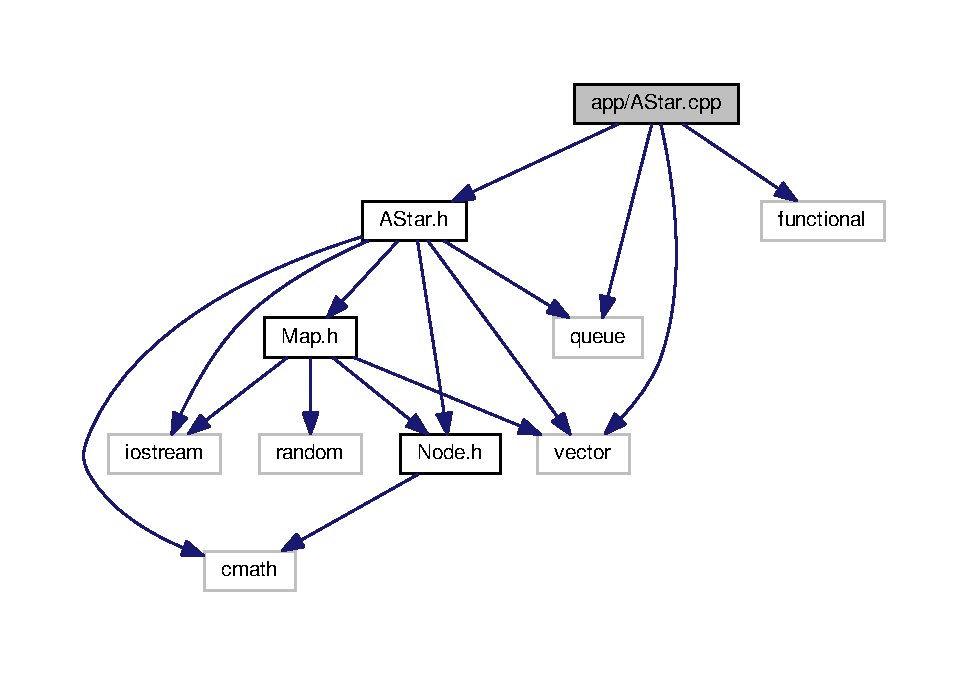
\includegraphics[width=350pt]{AStar_8cpp__incl}
\end{center}
\end{figure}
This graph shows which files directly or indirectly include this file\+:\nopagebreak
\begin{figure}[H]
\begin{center}
\leavevmode
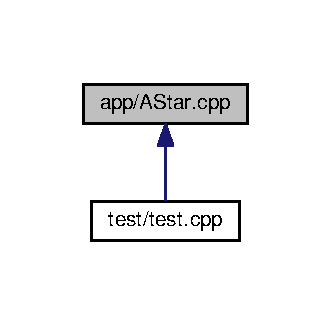
\includegraphics[width=159pt]{AStar_8cpp__dep__incl}
\end{center}
\end{figure}
\subsection*{Functions}
\begin{DoxyCompactItemize}
\item 
bool \hyperlink{AStar_8cpp_a6f3e17f3c0a31d1fae6b2569521a8e67}{operator$>$} (const \hyperlink{classNode}{Node} \&p, const \hyperlink{classNode}{Node} \&q)
\begin{DoxyCompactList}\small\item\em overloads the \textquotesingle{}$>$\textquotesingle{} operator \end{DoxyCompactList}\end{DoxyCompactItemize}


\subsection{Detailed Description}
Implements A$\ast$ algorithm. 

Defines path\+Finding function that find the path Defines function to overload \textquotesingle{}$>$\textquotesingle{} operator to implement minimum priority queue Defines constructor and destructor

\begin{DoxyAuthor}{Author}
Pranav Inani 
\end{DoxyAuthor}
\begin{DoxyCopyright}{Copyright}
2017 
\end{DoxyCopyright}


\subsection{Function Documentation}
\index{A\+Star.\+cpp@{A\+Star.\+cpp}!operator$>$@{operator$>$}}
\index{operator$>$@{operator$>$}!A\+Star.\+cpp@{A\+Star.\+cpp}}
\subsubsection[{\texorpdfstring{operator$>$(const Node \&p, const Node \&q)}{operator>(const Node &p, const Node &q)}}]{\setlength{\rightskip}{0pt plus 5cm}bool operator$>$ (
\begin{DoxyParamCaption}
\item[{const {\bf Node} \&}]{p, }
\item[{const {\bf Node} \&}]{q}
\end{DoxyParamCaption}
)}\hypertarget{AStar_8cpp_a6f3e17f3c0a31d1fae6b2569521a8e67}{}\label{AStar_8cpp_a6f3e17f3c0a31d1fae6b2569521a8e67}


overloads the \textquotesingle{}$>$\textquotesingle{} operator 

gives priority to node with greater total cosr


\begin{DoxyParams}{Parameters}
{\em p} & is a reference of a node \\
\hline
{\em q} & is a reference of a node\\
\hline
\end{DoxyParams}
\begin{DoxyReturn}{Returns}
true if the total cost of p is greater, else false 
\end{DoxyReturn}

\hypertarget{Map_8cpp}{}\section{app/\+Map.cpp File Reference}
\label{Map_8cpp}\index{app/\+Map.\+cpp@{app/\+Map.\+cpp}}


Implements map class.  


{\ttfamily \#include $<$Map.\+h$>$}\\*
{\ttfamily \#include $<$vector$>$}\\*
Include dependency graph for Map.\+cpp\+:\nopagebreak
\begin{figure}[H]
\begin{center}
\leavevmode
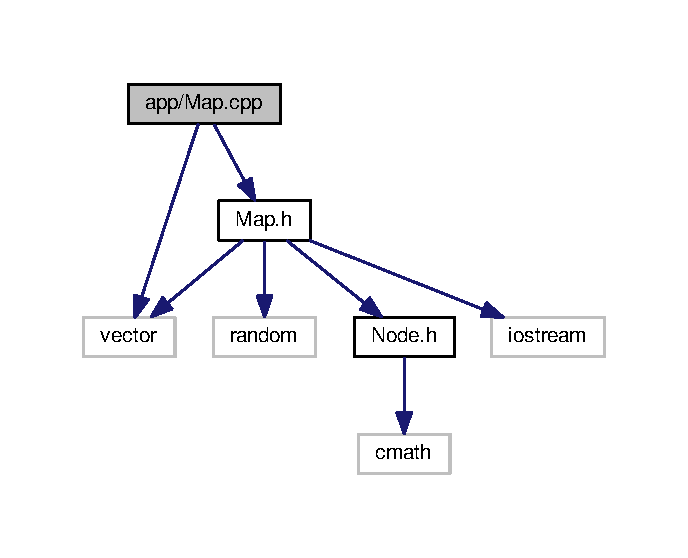
\includegraphics[width=330pt]{Map_8cpp__incl}
\end{center}
\end{figure}
This graph shows which files directly or indirectly include this file\+:\nopagebreak
\begin{figure}[H]
\begin{center}
\leavevmode
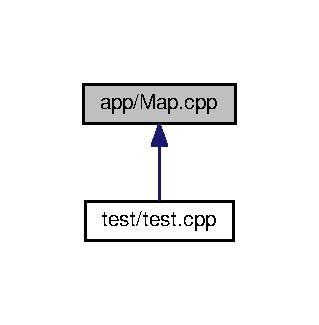
\includegraphics[width=153pt]{Map_8cpp__dep__incl}
\end{center}
\end{figure}


\subsection{Detailed Description}
Implements map class. 

defines create\+Map function that creates a map with obstacles defines print\+Map that prints the path found by the algortihm

\begin{DoxyAuthor}{Author}
Pranav Inani 
\end{DoxyAuthor}
\begin{DoxyCopyright}{Copyright}
2017 
\end{DoxyCopyright}

\hypertarget{Node_8cpp}{}\section{app/\+Node.cpp File Reference}
\label{Node_8cpp}\index{app/\+Node.\+cpp@{app/\+Node.\+cpp}}


Implements node class.  


{\ttfamily \#include $<$Node.\+h$>$}\\*
Include dependency graph for Node.\+cpp\+:\nopagebreak
\begin{figure}[H]
\begin{center}
\leavevmode
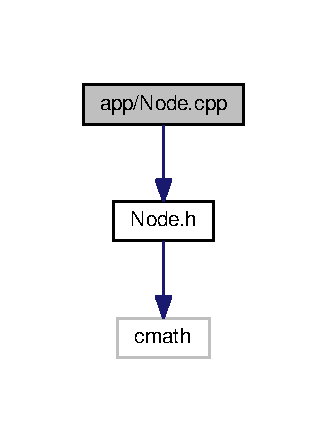
\includegraphics[width=157pt]{Node_8cpp__incl}
\end{center}
\end{figure}
This graph shows which files directly or indirectly include this file\+:\nopagebreak
\begin{figure}[H]
\begin{center}
\leavevmode
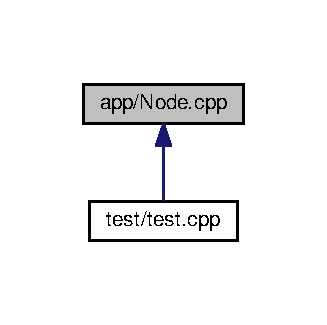
\includegraphics[width=157pt]{Node_8cpp__dep__incl}
\end{center}
\end{figure}


\subsection{Detailed Description}
Implements node class. 

Defines functions to compute heuristic, path cost and total cost Defines constructor and destructor

\begin{DoxyAuthor}{Author}
Pranav Inani 
\end{DoxyAuthor}
\begin{DoxyCopyright}{Copyright}
2017 
\end{DoxyCopyright}

\hypertarget{AStar_8h}{}\section{include/\+A\+Star.h File Reference}
\label{AStar_8h}\index{include/\+A\+Star.\+h@{include/\+A\+Star.\+h}}


Contains declarations for \hyperlink{classAStar}{A\+Star} class.  


{\ttfamily \#include $<$iostream$>$}\\*
{\ttfamily \#include $<$cmath$>$}\\*
{\ttfamily \#include $<$queue$>$}\\*
{\ttfamily \#include $<$vector$>$}\\*
{\ttfamily \#include $<$Node.\+h$>$}\\*
{\ttfamily \#include $<$Map.\+h$>$}\\*
Include dependency graph for A\+Star.\+h\+:\nopagebreak
\begin{figure}[H]
\begin{center}
\leavevmode
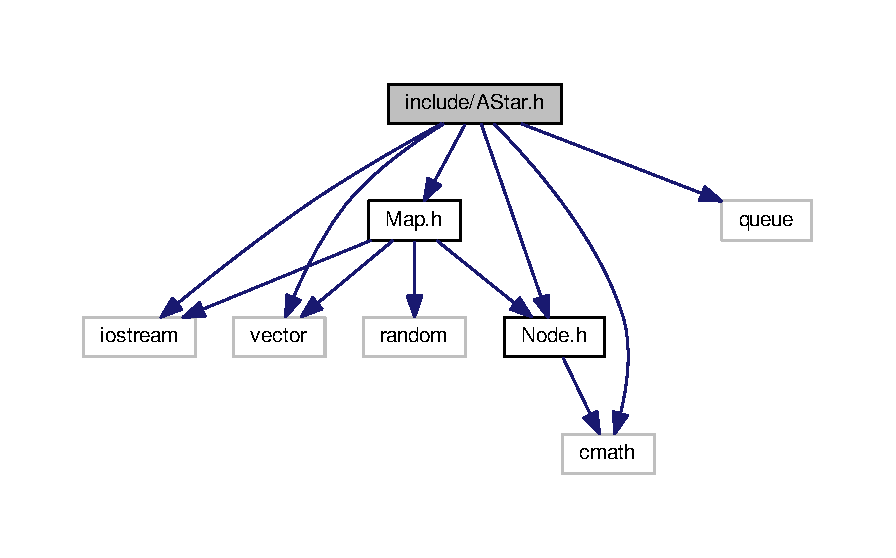
\includegraphics[width=350pt]{AStar_8h__incl}
\end{center}
\end{figure}
This graph shows which files directly or indirectly include this file\+:\nopagebreak
\begin{figure}[H]
\begin{center}
\leavevmode
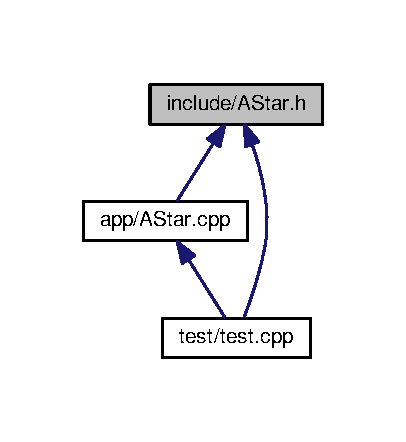
\includegraphics[width=195pt]{AStar_8h__dep__incl}
\end{center}
\end{figure}
\subsection*{Classes}
\begin{DoxyCompactItemize}
\item 
class \hyperlink{classAStar}{A\+Star}
\begin{DoxyCompactList}\small\item\em Defines the \hyperlink{classAStar}{A\+Star} class. \end{DoxyCompactList}\end{DoxyCompactItemize}


\subsection{Detailed Description}
Contains declarations for \hyperlink{classAStar}{A\+Star} class. 

Declares path\+Find functions that performs the implementation Declares start and end coordinates as private members Declares function to overload \textquotesingle{}$>$\textquotesingle{} operator Declares constructor and destructor of \hyperlink{classAStar}{A\+Star} class

\begin{DoxyAuthor}{Author}
Pranav Inani 
\end{DoxyAuthor}
\begin{DoxyCopyright}{Copyright}
2017 
\end{DoxyCopyright}

\hypertarget{Map_8h}{}\section{include/\+Map.h File Reference}
\label{Map_8h}\index{include/\+Map.\+h@{include/\+Map.\+h}}


Contains Declarations for \hyperlink{classMap}{Map} Class.  


{\ttfamily \#include $<$vector$>$}\\*
{\ttfamily \#include $<$random$>$}\\*
{\ttfamily \#include $<$Node.\+h$>$}\\*
{\ttfamily \#include $<$iostream$>$}\\*
Include dependency graph for Map.\+h\+:\nopagebreak
\begin{figure}[H]
\begin{center}
\leavevmode
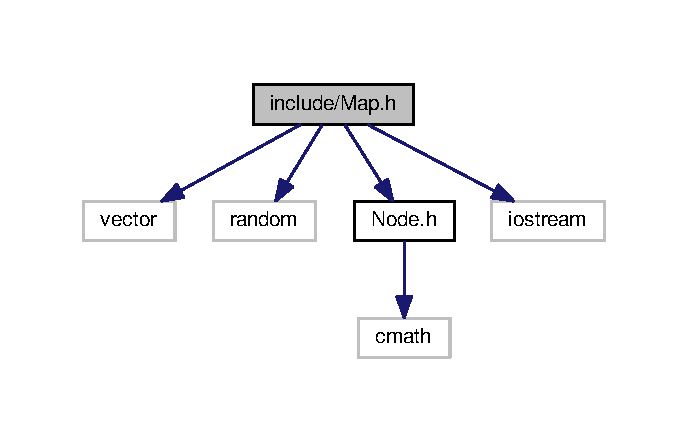
\includegraphics[width=330pt]{Map_8h__incl}
\end{center}
\end{figure}
This graph shows which files directly or indirectly include this file\+:\nopagebreak
\begin{figure}[H]
\begin{center}
\leavevmode
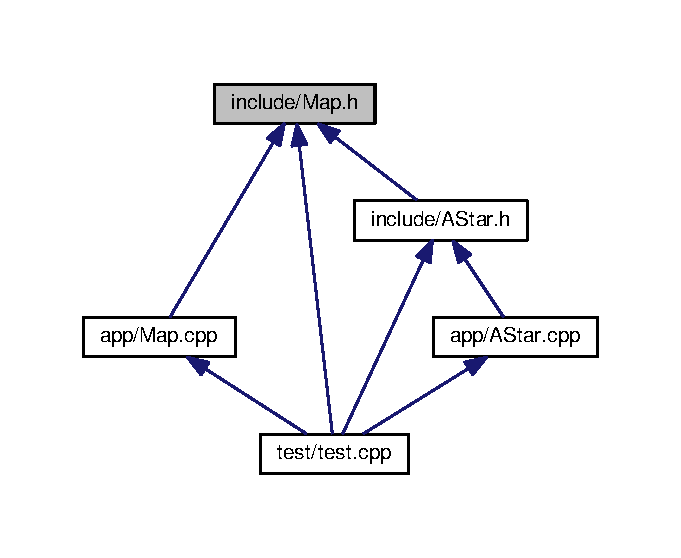
\includegraphics[width=327pt]{Map_8h__dep__incl}
\end{center}
\end{figure}
\subsection*{Classes}
\begin{DoxyCompactItemize}
\item 
class \hyperlink{classMap}{Map}
\begin{DoxyCompactList}\small\item\em Defines the \hyperlink{classMap}{Map} class. \end{DoxyCompactList}\end{DoxyCompactItemize}


\subsection{Detailed Description}
Contains Declarations for \hyperlink{classMap}{Map} Class. 

Declares create\+Map function that creates a map Declares print\+Path functions that prints the path

\begin{DoxyAuthor}{Author}
Pranav Inani 
\end{DoxyAuthor}
\begin{DoxyCopyright}{Copyright}
2017 
\end{DoxyCopyright}

\hypertarget{Node_8h}{}\section{include/\+Node.h File Reference}
\label{Node_8h}\index{include/\+Node.\+h@{include/\+Node.\+h}}


Contains declarations for \hyperlink{classNode}{Node} class.  


{\ttfamily \#include $<$cmath$>$}\\*
Include dependency graph for Node.\+h\+:\nopagebreak
\begin{figure}[H]
\begin{center}
\leavevmode
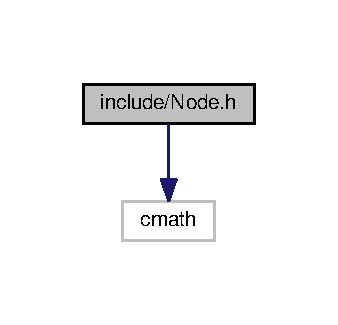
\includegraphics[width=162pt]{Node_8h__incl}
\end{center}
\end{figure}
This graph shows which files directly or indirectly include this file\+:\nopagebreak
\begin{figure}[H]
\begin{center}
\leavevmode
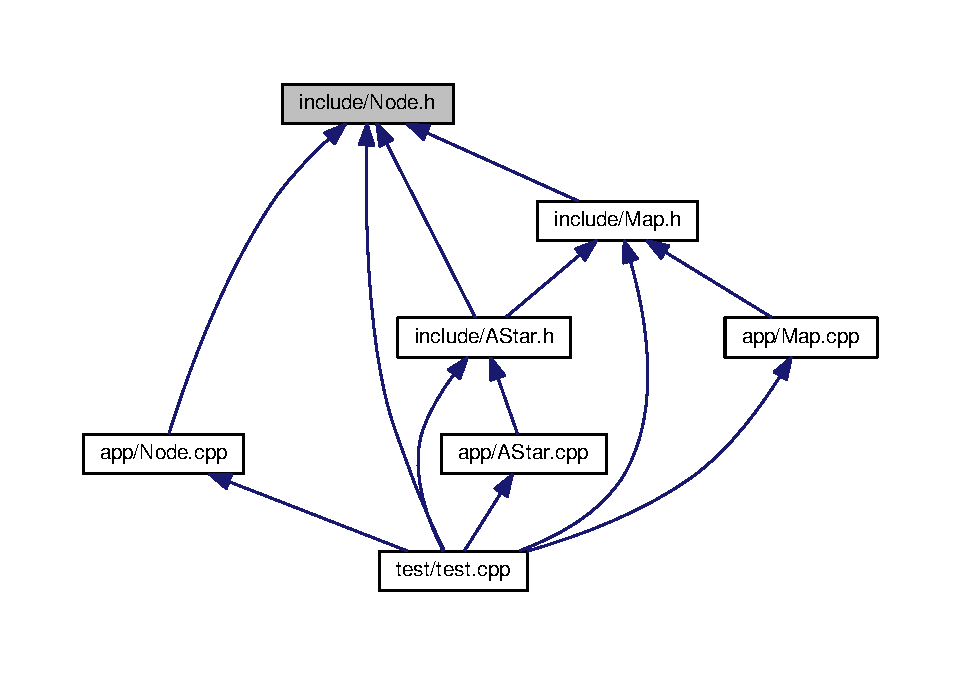
\includegraphics[width=350pt]{Node_8h__dep__incl}
\end{center}
\end{figure}
\subsection*{Classes}
\begin{DoxyCompactItemize}
\item 
class \hyperlink{classNode}{Node}
\begin{DoxyCompactList}\small\item\em Defines the \hyperlink{classNode}{Node} class. \end{DoxyCompactList}\end{DoxyCompactItemize}


\subsection{Detailed Description}
Contains declarations for \hyperlink{classNode}{Node} class. 

Declares x, y, total\+Cost and path\+Cost as public members Declares heuristic function that calculates Euclidian distance Declares g\+Cal that calculates path\+Cost Declares f\+Cal that calculates total cost Declares constructor and destructor

\begin{DoxyAuthor}{Author}
Pranav Inani 
\end{DoxyAuthor}
\begin{DoxyCopyright}{Copyright}
2017 
\end{DoxyCopyright}

\hypertarget{test_8cpp}{}\section{test/test.cpp File Reference}
\label{test_8cpp}\index{test/test.\+cpp@{test/test.\+cpp}}


Contains Unit tests.  


{\ttfamily \#include $<$gtest/gtest.\+h$>$}\\*
{\ttfamily \#include $<$vector$>$}\\*
{\ttfamily \#include \char`\"{}../include/\+Node.\+h\char`\"{}}\\*
{\ttfamily \#include \char`\"{}../app/\+Node.\+cpp\char`\"{}}\\*
{\ttfamily \#include \char`\"{}../include/\+A\+Star.\+h\char`\"{}}\\*
{\ttfamily \#include \char`\"{}../app/\+A\+Star.\+cpp\char`\"{}}\\*
{\ttfamily \#include \char`\"{}../include/\+Map.\+h\char`\"{}}\\*
{\ttfamily \#include \char`\"{}../app/\+Map.\+cpp\char`\"{}}\\*
Include dependency graph for test.\+cpp\+:\nopagebreak
\begin{figure}[H]
\begin{center}
\leavevmode
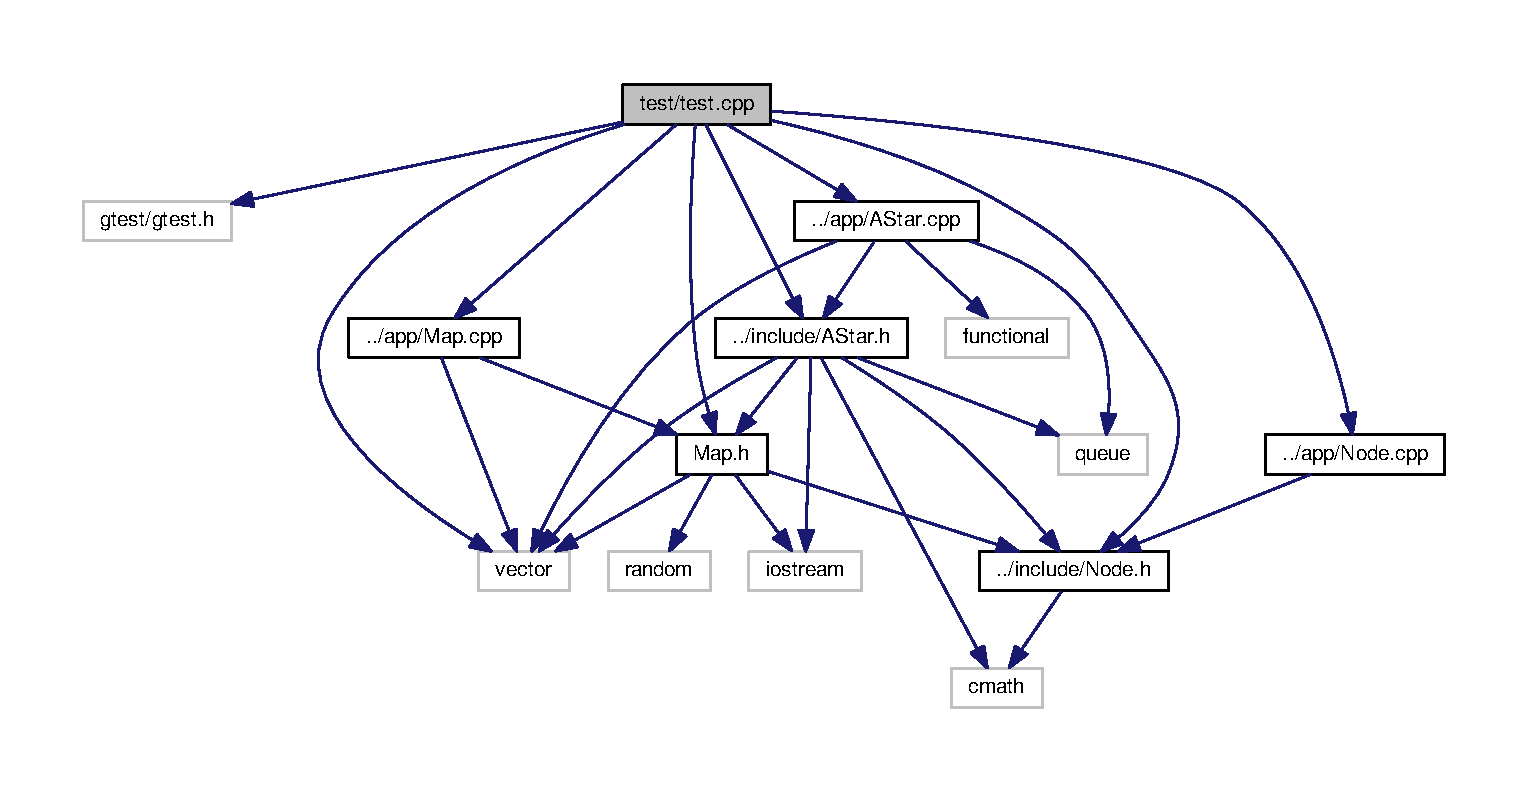
\includegraphics[width=350pt]{test_8cpp__incl}
\end{center}
\end{figure}
\subsection*{Functions}
\begin{DoxyCompactItemize}
\item 
\hyperlink{test_8cpp_a57cac6e439db434ca1213372c5f6b873}{T\+E\+ST} (Heuristic\+Test, Check\+Calculated\+Distance)
\begin{DoxyCompactList}\small\item\em Unit test for Heuristic Calculation. \end{DoxyCompactList}\item 
\hyperlink{test_8cpp_a2bb99463b6ac087913c231778e0b714c}{T\+E\+ST} (Path\+Cost\+Test, Check\+Path\+Cost\+Calculation)
\begin{DoxyCompactList}\small\item\em Unit test for path cost calculation. \end{DoxyCompactList}\item 
\hyperlink{test_8cpp_a9b0631f71faa4616d77d30304433b60b}{T\+E\+ST} (Total\+Cost\+Test, F\+Is\+Greater)
\begin{DoxyCompactList}\small\item\em Unit test total function cost calculation. \end{DoxyCompactList}\item 
\hyperlink{test_8cpp_a1036e70cf8f103cd4ded740c4ace372f}{T\+E\+ST} (Operator\+Test, Test\+Min\+PriorityQ)
\begin{DoxyCompactList}\small\item\em Unit test for checking the overloaded \textquotesingle{}$>$\textquotesingle{} operator. \end{DoxyCompactList}\item 
\hyperlink{test_8cpp_a59329afeb275aab7cb4f7a39168f2779}{T\+E\+ST} (Goal\+Blocked, Path\+Not\+Found)
\begin{DoxyCompactList}\small\item\em Unit test to check if goal node is blocked. \end{DoxyCompactList}\item 
\hyperlink{test_8cpp_a114fc18553609e0ae6fbbed847b320a0}{T\+E\+ST} (Start\+Walkable, Map\+Value\+Is\+One)
\begin{DoxyCompactList}\small\item\em Unit test to check if start node is walkable. \end{DoxyCompactList}\item 
\hyperlink{test_8cpp_a6cb5e3cfec6c4f38a6be2a24046fcf6d}{T\+E\+ST} (Path\+Found, Return\+One\+If\+Found)
\begin{DoxyCompactList}\small\item\em Unit test to check if path is found. \end{DoxyCompactList}\item 
\hyperlink{test_8cpp_a2c33759c44e5abe6f672de2017ff387f}{T\+E\+ST} (Path\+Not\+Found, Return\+Minus\+One\+If\+Not\+Found)
\begin{DoxyCompactList}\small\item\em Unit test to check if path is not found. \end{DoxyCompactList}\end{DoxyCompactItemize}


\subsection{Detailed Description}
Contains Unit tests. 

Defines several unit tests to check the correct behavior of various methods in \hyperlink{classNode}{Node}, \hyperlink{classMap}{Map} and \hyperlink{classAStar}{A\+Star} class

\begin{DoxyAuthor}{Author}
Pranav Inani 
\end{DoxyAuthor}
\begin{DoxyCopyright}{Copyright}
2017 
\end{DoxyCopyright}


\subsection{Function Documentation}
\index{test.\+cpp@{test.\+cpp}!T\+E\+ST@{T\+E\+ST}}
\index{T\+E\+ST@{T\+E\+ST}!test.\+cpp@{test.\+cpp}}
\subsubsection[{\texorpdfstring{T\+E\+S\+T(\+Heuristic\+Test, Check\+Calculated\+Distance)}{TEST(HeuristicTest, CheckCalculatedDistance)}}]{\setlength{\rightskip}{0pt plus 5cm}T\+E\+ST (
\begin{DoxyParamCaption}
\item[{Heuristic\+Test}]{, }
\item[{Check\+Calculated\+Distance}]{}
\end{DoxyParamCaption}
)}\hypertarget{test_8cpp_a57cac6e439db434ca1213372c5f6b873}{}\label{test_8cpp_a57cac6e439db434ca1213372c5f6b873}


Unit test for Heuristic Calculation. 

Checks if Heuristic function is returning the expected distance value \index{test.\+cpp@{test.\+cpp}!T\+E\+ST@{T\+E\+ST}}
\index{T\+E\+ST@{T\+E\+ST}!test.\+cpp@{test.\+cpp}}
\subsubsection[{\texorpdfstring{T\+E\+S\+T(\+Path\+Cost\+Test, Check\+Path\+Cost\+Calculation)}{TEST(PathCostTest, CheckPathCostCalculation)}}]{\setlength{\rightskip}{0pt plus 5cm}T\+E\+ST (
\begin{DoxyParamCaption}
\item[{Path\+Cost\+Test}]{, }
\item[{Check\+Path\+Cost\+Calculation}]{}
\end{DoxyParamCaption}
)}\hypertarget{test_8cpp_a2bb99463b6ac087913c231778e0b714c}{}\label{test_8cpp_a2bb99463b6ac087913c231778e0b714c}


Unit test for path cost calculation. 

Checks if the function is returning the expected value of path cost \index{test.\+cpp@{test.\+cpp}!T\+E\+ST@{T\+E\+ST}}
\index{T\+E\+ST@{T\+E\+ST}!test.\+cpp@{test.\+cpp}}
\subsubsection[{\texorpdfstring{T\+E\+S\+T(\+Total\+Cost\+Test, F\+Is\+Greater)}{TEST(TotalCostTest, FIsGreater)}}]{\setlength{\rightskip}{0pt plus 5cm}T\+E\+ST (
\begin{DoxyParamCaption}
\item[{Total\+Cost\+Test}]{, }
\item[{F\+Is\+Greater}]{}
\end{DoxyParamCaption}
)}\hypertarget{test_8cpp_a9b0631f71faa4616d77d30304433b60b}{}\label{test_8cpp_a9b0631f71faa4616d77d30304433b60b}


Unit test total function cost calculation. 

Checks if function is returning the expected value of the total function cost \index{test.\+cpp@{test.\+cpp}!T\+E\+ST@{T\+E\+ST}}
\index{T\+E\+ST@{T\+E\+ST}!test.\+cpp@{test.\+cpp}}
\subsubsection[{\texorpdfstring{T\+E\+S\+T(\+Operator\+Test, Test\+Min\+Priority\+Q)}{TEST(OperatorTest, TestMinPriorityQ)}}]{\setlength{\rightskip}{0pt plus 5cm}T\+E\+ST (
\begin{DoxyParamCaption}
\item[{Operator\+Test}]{, }
\item[{Test\+Min\+PriorityQ}]{}
\end{DoxyParamCaption}
)}\hypertarget{test_8cpp_a1036e70cf8f103cd4ded740c4ace372f}{}\label{test_8cpp_a1036e70cf8f103cd4ded740c4ace372f}


Unit test for checking the overloaded \textquotesingle{}$>$\textquotesingle{} operator. 

Checks if the node with greater total cost is given priority \index{test.\+cpp@{test.\+cpp}!T\+E\+ST@{T\+E\+ST}}
\index{T\+E\+ST@{T\+E\+ST}!test.\+cpp@{test.\+cpp}}
\subsubsection[{\texorpdfstring{T\+E\+S\+T(\+Goal\+Blocked, Path\+Not\+Found)}{TEST(GoalBlocked, PathNotFound)}}]{\setlength{\rightskip}{0pt plus 5cm}T\+E\+ST (
\begin{DoxyParamCaption}
\item[{Goal\+Blocked}]{, }
\item[{Path\+Not\+Found}]{}
\end{DoxyParamCaption}
)}\hypertarget{test_8cpp_a59329afeb275aab7cb4f7a39168f2779}{}\label{test_8cpp_a59329afeb275aab7cb4f7a39168f2779}


Unit test to check if goal node is blocked. 

If goal node is blocked path won\textquotesingle{}t be found \index{test.\+cpp@{test.\+cpp}!T\+E\+ST@{T\+E\+ST}}
\index{T\+E\+ST@{T\+E\+ST}!test.\+cpp@{test.\+cpp}}
\subsubsection[{\texorpdfstring{T\+E\+S\+T(\+Start\+Walkable, Map\+Value\+Is\+One)}{TEST(StartWalkable, MapValueIsOne)}}]{\setlength{\rightskip}{0pt plus 5cm}T\+E\+ST (
\begin{DoxyParamCaption}
\item[{Start\+Walkable}]{, }
\item[{Map\+Value\+Is\+One}]{}
\end{DoxyParamCaption}
)}\hypertarget{test_8cpp_a114fc18553609e0ae6fbbed847b320a0}{}\label{test_8cpp_a114fc18553609e0ae6fbbed847b320a0}


Unit test to check if start node is walkable. 

Asserts that start node should never be an obstacle \index{test.\+cpp@{test.\+cpp}!T\+E\+ST@{T\+E\+ST}}
\index{T\+E\+ST@{T\+E\+ST}!test.\+cpp@{test.\+cpp}}
\subsubsection[{\texorpdfstring{T\+E\+S\+T(\+Path\+Found, Return\+One\+If\+Found)}{TEST(PathFound, ReturnOneIfFound)}}]{\setlength{\rightskip}{0pt plus 5cm}T\+E\+ST (
\begin{DoxyParamCaption}
\item[{Path\+Found}]{, }
\item[{Return\+One\+If\+Found}]{}
\end{DoxyParamCaption}
)}\hypertarget{test_8cpp_a6cb5e3cfec6c4f38a6be2a24046fcf6d}{}\label{test_8cpp_a6cb5e3cfec6c4f38a6be2a24046fcf6d}


Unit test to check if path is found. 

If a path is found print\+Path function should return 1 \index{test.\+cpp@{test.\+cpp}!T\+E\+ST@{T\+E\+ST}}
\index{T\+E\+ST@{T\+E\+ST}!test.\+cpp@{test.\+cpp}}
\subsubsection[{\texorpdfstring{T\+E\+S\+T(\+Path\+Not\+Found, Return\+Minus\+One\+If\+Not\+Found)}{TEST(PathNotFound, ReturnMinusOneIfNotFound)}}]{\setlength{\rightskip}{0pt plus 5cm}T\+E\+ST (
\begin{DoxyParamCaption}
\item[{Path\+Not\+Found}]{, }
\item[{Return\+Minus\+One\+If\+Not\+Found}]{}
\end{DoxyParamCaption}
)}\hypertarget{test_8cpp_a2c33759c44e5abe6f672de2017ff387f}{}\label{test_8cpp_a2c33759c44e5abe6f672de2017ff387f}


Unit test to check if path is not found. 

If a path is not found print\+Path function should return -\/1 
%--- End generated contents ---

% Index
\backmatter
\newpage
\phantomsection
\clearemptydoublepage
\addcontentsline{toc}{chapter}{Index}
\printindex

\end{document}
